\section{PETALO Scanners}
\label{sec.pets}


\begin{figure}[!htb]
	\centering
	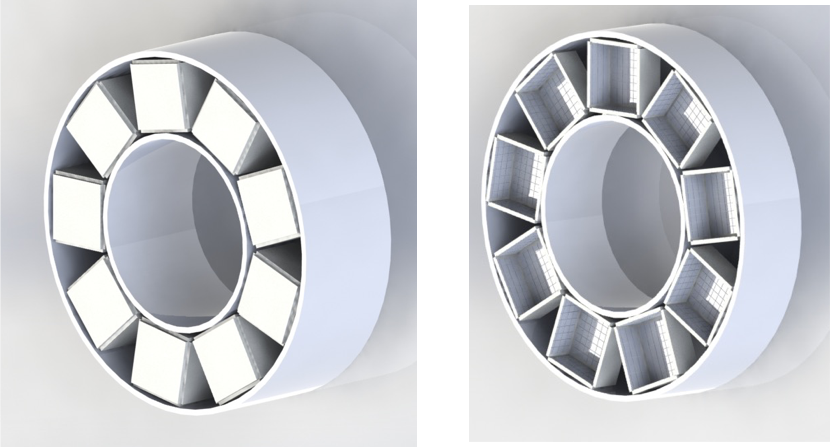
\includegraphics[scale=0.4]{img/SAP.png}
	\caption{\label{fig.smallPet} A conceptual drawing of a small brain PET, based in 9 LXSC. }
\end{figure}

As we have shown in previous sections, the excellent energy resolution, excellent CRT and good spatial resolution of the LXSC makes it the cornerstone of a number of PET systems.  For example:

\begin{enumerate}
\item {\bf A ``full body'' PET} application (e.g, a large PET device, comprising several rings of large diameter, covering the full torso of the patient), needs to be optimized for cost, and could benefit for the most sparse configuration (LXSC2 of $5\times5\times5$~cm$^3$~ with 32 SiPMs of 6 mm$^2$~per face).
\item {\bf A ``small animal'' PET} application, which intends to reconstruct images of the small organs of test animals such as mice, needs to be optimized for spatial resolution, and could be based in a LXSC2 fully instrumented with small SiPMs (of 3 mm$^2$~or smaller). The size of the box should be adjusted to the PET smallish diameter (to keep good packing) and the thickness of the box could be reduced to 2 cm, to optimize spatial resolution (trading it for efficiency which could be less critical for this application).
\item {\bf A ``brain scan'' PET} application, requires less modules than a full body PET and does not require a resolution as good as small animal PET, thus it could be based in an LXSC2 of a size intermediate between the small animal PET and the full body PET.
\end{enumerate}

%
% It has better energy and spatial resolutions than PETs currently in the market and it is also cheaper. Figure \ref{fig.smallPet} shows the design of a small brain PET using LXSC.
%
%In this section we discuss another two important features that PETALO potentially has: TOF-PET capability and NMR compatibility.
\subsubsection*{TOF application}

The quick decay time of xenon and the fast circuitry available in modern SiPMs offers an extraordinary potential for TOF applications. About 2.5\% of the photons are emitted in LXe in the first 50 ps after the interaction. The SiPM recording more signal in one event sees typically  2\% of the total photoelectrons (pes), and therefore it records 5 pes in the first 50 ps, enough to trigger a signal. For comparison, one nanosecond is needed in LSO to emit 2.5\% of the photons. Commercial TOF-PET systems based in LYSO (a proprietary version of LSO) have achieved a system time resolution of 600 ps. Since LXe features {\em both} higher light yield and much faster time response, a system resolution at the level or better than 200 ps appears possible. Thus, PETALO could represent a breakthrough in the field of PET-TOF. 

\subsubsection*{MRI compatibility}

Magnetic Resonante Imaging (MRI) is a medical imaging technique that shows anatomical features using an NMR apparatus. There is strong interest in building a MRI-compatible PET scanner capable of acquiring PET images simultaneously with MRI images and, therefore, combining anatomical and functional information.

The main issue is that an MRI requires strong magnetic fields and, hence, is not compatible with current PET systems due to the use of photomultiplier tubes (PMT), which will not function under high magnetic fields.

On the other hand, the LXSC is built using non-magnetic materials, and unlike PMTs, SiPMs can operate in very high magnetic fields. Thus, PETALO can operate inside the very intense magnetic field generated by NMR devices. Furthermore, a NMR apparatus requires a large cryostat which can also accommodate the LXSC modules that make up PETALO. The technology offers, therefore, the possibility of building a fully MRI compatible device.  

